\documentclass[final,3p,times]{elsarticle}

%% ==========================================
%% Packages
%% ==========================================
\usepackage{amssymb}
\usepackage{amsmath}
\usepackage{graphicx}
\usepackage{booktabs}
\usepackage{algorithm}
\usepackage{algorithmicx}
\usepackage{algpseudocode}
\usepackage{bm}
\usepackage{hyperref}
\usepackage{color}
\usepackage{tikz}
\usetikzlibrary{arrows.meta,positioning}

%% ==========================================
%% Journal info
%% ==========================================
\journal{Pattern Recognition Letters}

\begin{document}

\begin{frontmatter}

%% ==========================================
%% Title
%% ==========================================
\title{Reliability-Aware RGB-D Terrain Clustering for Robotic Guide Dogs under Sensor Degradation}

%% ==========================================
%% Authors & Affiliations
%% ==========================================
\author[inst1]{Dong Yan}
\author[inst1]{Yufeng Xiao\corref{cor1}}
\ead{yufeng.xiao@swust.edu.cn}
\cortext[cor1]{Corresponding author}

\author[inst1]{Zhenyu Ren}
\author[inst1]{Yaolong Zhao}

\affiliation[inst1]{
    organization={Special Environment Robotics Laboratory, Southwest University of Science and Technology},
    city={Mianyang},
    country={China}
}

%% ==========================================
%% Abstract
%% ==========================================
\begin{abstract}
Robotic guide dogs must recognize terrain while camera and depth streams degrade. We present a reliability-aware RGB-D terrain clustering method with per-sample sensor-health estimation and a calibrated online readout. Per-sample reliability scores are computed from exposure, contrast, sharpness, depth validity, and depth smoothness; softmax weights define a weighted concatenation that is clustered by reliability-weighted multi-view $K$-means. Clusters are mapped to terrain classes by majority vote on a small labelled calibration set, and online samples are assigned to the nearest cluster centroid, so clustering drives the terrain label used by a semantic-adaptive particle filter (SAPF). Silhouette scores are used only for evaluation. On a corrected NYU Depth V2 pilot subset (17 images per class), the method reaches $71.1\%$ clustering accuracy and $38.3\%$ NMI on clean data and $60.0\%$ accuracy at the most severe injected degradation, the numerically highest ACC among the evaluated methods. On a 351-sample ROS/Gazebo street scene, the cluster readout obtains $77.8\%$ under blocked cross-validation, $90.1\pm1.0\%$ online, and $77.6\pm1.6\%$ under mixed sensor degradation. A fair comparison including a fixed large-covariance PF shows clear gains over the standard PF, while SAPF is comparable to the large-covariance baseline; a shuffled-label control is worse on the clean run. A zero-shot cross-illumination check drops to 73.3\%, showing that the in-scene result is not cross-domain generalization. The study is limited to a pilot NYU subset, kinematic Gazebo locomotion, a simulated exteroceptive pose, and in-scene calibration.
\end{abstract}

%% ==========================================
%% Keywords
%% ==========================================
\begin{keyword}
Reliability-aware multi-view clustering \sep RGB-D terrain perception \sep Sensor degradation \sep Cluster-to-terrain calibration \sep Semantic-adaptive particle filter \sep Robotic guide dog
\end{keyword}

\end{frontmatter}

%% ==========================================
%% 1. Introduction
%% ==========================================
\section{Introduction}
\label{sec:intro}
Robotic guide dogs are expected to accompany visually impaired users through sidewalks, tactile paving, obstacles, and staircases. Unlike vehicles operating on structured roads, a quadrupedal guide dog must interpret fine-grained terrain semantics while maintaining a reliable 6-DoF pose estimate in the presence of locomotion-induced vibration, foot slip, and sensor degradation. A single sensing modality is fragile in this setting: vision is affected by overexposure, motion blur, and illumination changes, whereas depth or LiDAR measurements can become sparse or corrupted by multipath reflections and dropouts.

A fixed fusion rule is not sufficient in this setting. When one modality is severely degraded, naive concatenation or a fixed weighting can propagate corrupted features into the downstream estimator. Equally important, the semantic label produced by the perception front end is rarely connected to the process noise of the state estimator: a conventional particle filter uses the same motion covariance on flat ground and on stairs, which can cause delayed elevation response or $z$-axis drift.

This paper therefore treats terrain clustering as the primary problem and state estimation as a downstream validation of the cluster output. The proposed front end, called reliability-aware adaptive heterogeneous physical feature fusion (RA-AHPFF), differs from a conventional silhouette-weighted pipeline in three respects. First, the modality weights are computed from per-sample sensor-health indicators rather than from silhouette scores, which removes the circular dependency between clustering and weighting. Second, the two descriptor blocks are combined by weighted concatenation in a common standardized space; PCA projections from different sensor spaces are not added. Third, the online terrain label is obtained by assigning the current descriptor to a cluster centroid and reading out the terrain class of that cluster, so that clustering is actually used by the robot rather than being an offline ablation only.

The main contributions are:
\begin{itemize}
    \item We formulate a reliability-aware multi-view clustering front end with per-sample visual and depth health indicators, softmax modality weights, weighted concatenation, and reliability-weighted multi-view $K$-means. The weights are computed independently of the clustering objective, and silhouette scores are used only for evaluation.
    \item We connect clustering to the online system through a cluster-to-terrain calibration step. A small labelled set is used only to name the clusters; online samples are assigned to the nearest centroid and the mapped terrain label is published to the state estimator. A supervised classifier is retained only as an upper-bound comparison.
    \item We provide a fair downstream evaluation of the semantic-adaptive particle filter against odometry, a standard particle filter, a fixed large-covariance particle filter, an extended Kalman filter, an oracle-label variant, and a shuffled-label variant. The comparison is repeated over multiple runs and uses a reduced-rate exteroceptive pose stream with outage windows rather than an idealized 50~Hz absolute pose.
    \item We report the performance and the limitations of the resulting system on a corrected NYU Depth V2 pilot subset, a 351-sample in-scene RGB-D calibration set, and a ROS/Gazebo Go1 street scene. The code and the processed data are available from the corresponding author upon reasonable request.
\end{itemize}

%% ==========================================
%% 2. Related Work
%% ==========================================
\section{Related Work}
\label{sec:related_work}
\subsection{Sensor-Driven Assistive Navigation and Guide Dog Robots}
Sensor-driven assistive technologies have been developed around smartphones, electronic white canes, and wearable devices \cite{patel2024review, wang2026design, ye2016co}. The Virtual Guide Dog uses onboard sensors and the NTCIP protocol to communicate with traffic controllers at intersections \cite{zhong2020virtual}. With the progress of legged robotics, quadrupedal platforms have been explored as physical guide dogs. The iDog system uses AI and edge computing for real-time audio alerts \cite{chen2024idog}, and Hwang et al. developed a guide dog robot with a rigid harness and a semantics-aware local planner \cite{hwang2022system}. Physical human-robot interaction and locomotion comfort are also critical: Fan et al. proposed a force-compliance MPC framework for interactive navigation \cite{fan2024force}, and Yu et al. emphasized quiet and stable locomotion for acoustic situational awareness \cite{yu2025human}. These systems demonstrate the importance of robust perception and state estimation, but they typically use deterministic or loosely coupled fusion and do not connect terrain semantics to the process noise of a probabilistic filter.

\subsection{Multi-View Clustering and Reliability-Aware Fusion}
Multi-view clustering (MVC) provides a natural formulation for combining heterogeneous sensor views \cite{wang2024self, chowdhury2025deep, fang2023comprehensive}. Graph-regularized nonnegative matrix factorization embeds local geometric structure and orthogonal constraints \cite{zhang2018multi}; spectral analysis with local refinement captures fine-grained visual topology \cite{xu2021multi}; and angular metric learning can produce tighter class boundaries \cite{shi2023deep}. Continual and incomplete-view methods update consensus coefficients or handle missing samples \cite{wan2023fast, liang2022incomplete}, and auto-weighted binary MVC learns view and sample weights jointly \cite{houfar2023automatically}. Most of these methods are designed for offline or soft-real-time clustering and assume that each view is available at test time. In a robotic system, the reliability of a view changes from frame to frame, so a fixed view weight is not sufficient. Our approach follows the reliability-weighting idea but keeps the descriptor set small and interpretable, and it explicitly calibrates clusters to terrain classes so that the result can be used online.

\subsection{Semantic-Aware State Estimation}
Particle filters are widely used for non-linear, multi-modal state estimation \cite{thrun2005probabilistic}. In legged and assistive robots, process and observation noise are often tuned for a single terrain type, which is inadequate when the robot transitions between flat ground, tactile paving, obstacles, and stairs. Semantic-aware estimation addresses this by using a terrain label to modulate the motion or observation model \cite{cadena2016past, miki2022learning}. Our SAPF follows this idea in a deliberately simple form: a discrete terrain label changes the diagonal process covariance, and the filter uses systematic resampling with an effective-sample-size trigger. We do not claim a new filtering algorithm; the purpose of the filter study is to test whether the cluster output is useful downstream and to compare it with strong fixed-covariance baselines.

%% ==========================================
%% 3. Methodology
%% ==========================================
\section{Methodology}
\label{sec:methodology}
\begin{figure}[t]
\centering
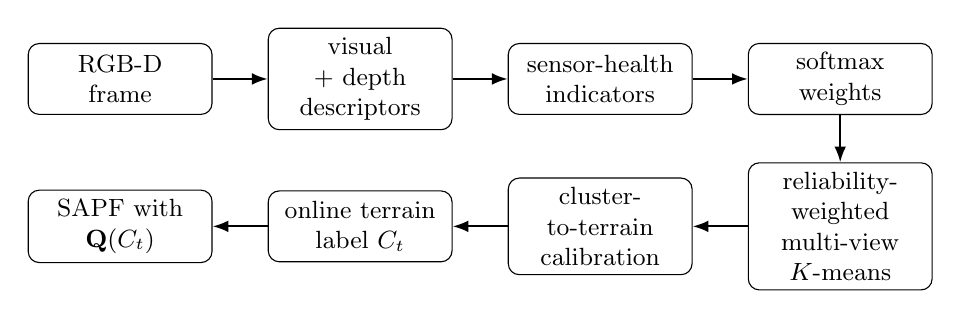
\begin{tikzpicture}[
    node distance=6mm and 7mm,
    box/.style={draw, rounded corners, align=center, font=\small, minimum height=9mm, text width=21mm},
    arrow/.style={-{Latex[length=2mm]}, thick}
]
\node[box] (rgbd) {RGB-D\\frame};
\node[box, right=of rgbd] (desc) {visual + depth\\descriptors};
\node[box, right=of desc] (health) {sensor-health\\indicators};
\node[box, right=of health] (weights) {softmax\\weights};
\node[box, below=of weights] (cluster) {reliability-weighted\\multi-view $K$-means};
\node[box, left=of cluster] (map) {cluster-to-terrain\\calibration};
\node[box, left=of map] (label) {online terrain\\label $C_t$};
\node[box, left=of label] (sapf) {SAPF with\\$\mathbf{Q}(C_t)$};
\draw[arrow] (rgbd) -- (desc);
\draw[arrow] (desc) -- (health);
\draw[arrow] (health) -- (weights);
\draw[arrow] (weights) -- (cluster);
\draw[arrow] (cluster) -- (map);
\draw[arrow] (map) -- (label);
\draw[arrow] (label) -- (sapf);
\end{tikzpicture}
\caption{Overview of the revised pipeline. The health indicators define per-sample modality weights; clustering is performed in the weighted descriptor space; the cluster-to-terrain mapping supplies the online label used by the SAPF.}
\label{fig:pipeline}
\end{figure}

The framework consists of a reliability-aware clustering front end and a 6-DoF SAPF back end (Fig.~\ref{fig:pipeline}). The front end produces a terrain label $C_t$; the back end uses $C_t$ to select the process covariance. The front end is trained once from a calibration set and then runs online.

\subsection{Interpretable RGB-D Descriptors}
\label{subsec:descriptors}
Let $\mathbf{X}^{(v)}_t$ and $\mathbf{X}^{(d)}_t$ denote the visual and depth observations. We extract interpretable descriptors rather than learned embeddings. The visual descriptor contains Canny edge density, Laplacian variance, mean and standard deviation of intensity, mean and standard deviation of gradient magnitude, intensity entropy, and, in the online RGB version, mean RGB values, mean saturation, and yellow/red fractions. The depth descriptor contains mean, standard deviation, minimum, maximum, 25th and 75th percentiles, depth span, mean absolute Sobel responses, mean gradient magnitude, and the ratio of valid depth pixels in the region of interest.

For NYU Depth V2, descriptors are computed inside the annotated object mask. For the RGB-D robot, they are computed inside a fixed lower-central region of interest $(0.15,0.85)\times(0.35,0.98)$ in normalized image coordinates. The visual block has 7 dimensions in the NYU experiment and 13 dimensions online; the depth block has 11 dimensions. The two blocks are standardized separately with statistics fitted on the calibration set.

\subsection{Per-Sample Sensor Health and Modality Weights}
\label{subsec:weights}
The key change relative to silhouette-weighted fusion is that the weights depend on observable sensor quality, not on the clustering result. The visual health score is
\begin{equation}
s_v = 0.32 e + 0.24 c + 0.20 h + 0.12 g + 0.06 \epsilon + 0.06 \kappa,
\label{eq:sv}
\end{equation}
where intensity is normalized to $[0,1]$ and gradients are normalized by 255. The components are
\begin{equation}
\begin{aligned}
e &= \operatorname{clip}(1-2|\mu_I-0.5|,0,1), \\
c &= \operatorname{clip}(\sigma_I/0.28,0,1), \\
h &= L/(L+40), \\
g &= \operatorname{clip}(\bar{G}/0.20,0,1), \\
\epsilon &= H/3, \\
\kappa &= \operatorname{clip}(d/0.08,0,1),
\end{aligned}
\label{eq:visual_terms}
\end{equation}
with mean intensity $\mu_I$, intensity standard deviation $\sigma_I$, Laplacian variance $L$, mean gradient magnitude $\bar{G}$, 8-bin intensity entropy $H$ in bits (hence the normalization by 3), and Canny edge density $d$. The visual reliability is $q_v=\sigma(5(s_v-0.45))$, where $\sigma(\cdot)$ is the logistic function.

The depth health score is
\begin{equation}
s_d = 0.50 r + 0.25 \omega + 0.15 \rho + 0.10 \gamma,
\label{eq:sd}
\end{equation}
where $r=N_{\mathrm{valid}}/N_{\mathrm{ROI}}\in[0,1]$ is the valid-pixel ratio, $\bar{D}$ is the mean depth in metres, and $\bar{G}_d$ is the mean depth-gradient magnitude. The terms are
\begin{equation}
\begin{aligned}
\bar{D} &= \max(\mu_D,10^{-6}), \\
\omega &= 1/(1+6\bar{G}_d/\bar{D}), \\
\rho &= \operatorname{clip}\!\left(\frac{D_{\max}-D_{\min}}{1.2\bar{D}},0,1\right), \\
\gamma &= 1-\exp(-\bar{D}/0.6).
\end{aligned}
\label{eq:depth_terms}
\end{equation}
The spread upper bound $1.2\bar{D}$ is a relative measure, so it adapts to the working range instead of using an absolute metre threshold. If no valid depth pixel is available ($r=0$), the depth reliability is set to zero and the sample receives zero depth weight. The depth reliability is $q_d=\sigma(5(s_d-0.45))$. The coefficients are fixed from the sensor model and are not fitted to the terrain labels.

Given $q_v$ and $q_d$, the modality weights are
\begin{equation}
w_v = \frac{\exp(\lambda q_v)}{\exp(\lambda q_v)+\exp(\lambda q_d)},
\qquad
w_d = 1-w_v,
\label{eq:weights}
\end{equation}
with $\lambda=4$ in all experiments. Because both reliabilities lie in $(0,1)$, the weights are well defined, non-negative, and sum to one. Unlike the previous silhouette ratio $s_1/(s_1+s_2)$, this construction cannot produce a negative or unbounded weight.

The standardized descriptor blocks are combined by weighted concatenation:
\begin{equation}
\mathbf{z}_t =
\left[
\sqrt{w_v}\,\tilde{\mathbf{z}}^{(v)}_t,\;
\sqrt{w_d}\,\tilde{\mathbf{z}}^{(d)}_t
\right],
\label{eq:fusion}
\end{equation}
where $\tilde{\mathbf{z}}^{(v)}$ and $\tilde{\mathbf{z}}^{(d)}$ are the per-view standardized descriptors. The blocks remain in their own coordinate systems; no PCA score from one view is added to a PCA score from the other view.

\subsection{Per-Sample Reliability-Weighted Multi-View $K$-Means}
\label{subsec:rwkmeans}
For a calibration set of $n$ samples, let $\mathbf{z}^{(v)}_i$ and $\mathbf{z}^{(d)}_i$ be the standardized views, and let $w_{vi},w_{di}$ be their weights. We minimize the weighted within-cluster objective
\begin{equation}
J = \sum_{k=1}^{K}\sum_{i\in \mathcal{C}_k}
\left(
w_{vi}\|\mathbf{z}^{(v)}_i-\mathbf{c}^{(v)}_k\|^2
+
w_{di}\|\mathbf{z}^{(d)}_i-\mathbf{c}^{(d)}_k\|^2
\right),
\label{eq:objective}
\end{equation}
where $\mathcal{C}_k$ is the set of samples assigned to cluster $k$. The assignment step uses the weighted distance in \eqref{eq:objective}, and the centroid update is the weighted mean
\begin{equation}
\mathbf{c}^{(v)}_k =
\frac{\sum_{i\in\mathcal{C}_k} w_{vi}\mathbf{z}^{(v)}_i}
{\sum_{i\in\mathcal{C}_k} w_{vi}},
\qquad
\mathbf{c}^{(d)}_k =
\frac{\sum_{i\in\mathcal{C}_k} w_{di}\mathbf{z}^{(d)}_i}
{\sum_{i\in\mathcal{C}_k} w_{di}}.
\label{eq:centroid}
\end{equation}
Because the weights are per-sample, this is a per-sample reliability-weighted variant, not ordinary $K$-means on one fixed weighted concatenation: the weighted concatenation changes across samples, and the centroid update in \eqref{eq:centroid} is the weighted mean of each view. We therefore call it per-sample reliability-weighted multi-view $K$-means (RW-MVK). Initialization uses $K$-means on the weighted concatenation \eqref{eq:fusion}; an empty cluster is reinitialized at the sample with the largest minimum distance to the current centroids. Algorithm~\ref{alg:rwkmeans} summarizes the procedure.

\begin{algorithm}[t]
\caption{Per-sample reliability-weighted multi-view $K$-means}
\label{alg:rwkmeans}
\begin{algorithmic}[1]
\Require standardized views $\{\mathbf{z}_i^{(v)},\mathbf{z}_i^{(d)}\}_{i=1}^{n}$, reliabilities $\{q_{vi},q_{di}\}$, clusters $K$, temperature $\lambda$, maximum iterations $T$, tolerance $\epsilon$
\State Compute $w_{vi},w_{di}$ from \eqref{eq:weights}.
\State Initialize centroids by $K$-means on $[\sqrt{w_{vi}}\mathbf{z}_i^{(v)},\sqrt{w_{di}}\mathbf{z}_i^{(d)}]$.
\For{$t=1$ to $T$}
    \State Assign each sample to the cluster with the minimum weighted distance in \eqref{eq:objective}.
    \State Update the two view centroids by \eqref{eq:centroid}.
    \If{a cluster is empty}
        \State Reinitialize its centroid at the sample with the largest minimum distance.
    \EndIf
    \State Compute the objective \eqref{eq:objective}; stop if its relative change is below $\epsilon$.
\EndFor
\State \Return cluster labels and centroids.
\end{algorithmic}
\end{algorithm}

The number of clusters is written as $K=rC$, where $C$ is the number of terrain classes and $r$ is an over-clustering factor. In the unsupervised NYU benchmark we use $r=1$ so that the clustering result is directly comparable to the number of annotated classes. In the calibrated online readout we use $r=8$ for the four-class RGB-D deployment ($K=32$) and $r=3$ for the three-class pilot readout ($K=9$). Over-clustering captures within-class appearance modes, such as different floor textures or stair viewpoints; each cluster is still mapped to a single terrain class by the calibration step below. The values of $r$ are calibration hyperparameters and are not selected using the evaluation labels.

\subsection{Cluster-to-Terrain Calibration and Online Readout}
\label{subsec:readout}
Let $\ell_i$ be the cluster index of calibration sample $i$ and $y_i$ its terrain class. For each cluster $k$, the class is chosen by majority vote:
\begin{equation}
m_k = \arg\max_{c\in\{1,\dots,C\}}
\sum_{i:\ell_i=k}\mathbf{1}[y_i=c].
\label{eq:mapping}
\end{equation}
Clusters without labelled samples are assigned to the global majority class. This step uses labels only to name clusters; it does not train a discriminative classifier.

At run time, the current descriptor is standardized with the stored per-view scalers, its reliability weights are computed from \eqref{eq:weights}, and the sample is assigned to the nearest centroid under the weighted distance. The published terrain label is $\hat{C}_t=m_{\hat{k}}$, where $\hat{k}$ is the assigned cluster. The confidence is the softmax of the negative cluster distances. A short majority filter over the last five predictions suppresses isolated label flips. A supervised ExtraTrees classifier is retained only as an upper-bound comparison in Section~\ref{subsec:go1_cluster}; it is not used in the online pipeline.

\subsection{Semantic-Adaptive Particle Filter}
\label{subsec:sapf}
The state is $\mathbf{x}_t = [p_x,p_y,p_z,\phi,\theta,\psi]^T$, where $\phi,\theta,\psi$ are roll, pitch, and yaw. The filter maintains $N$ particles $\{\mathbf{x}^{[i]}_t,w^{[i]}_t\}_{i=1}^{N}$.

\subsubsection{Motion Model and Semantic Covariance}
The state transition is
\begin{equation}
    \mathbf{x}^{[i]}_t = \mathbf{x}^{[i]}_{t-1} + \mathbf{u}_t + \bm{\epsilon}_t(C_t),
    \quad \bm{\epsilon}_t \sim \mathcal{N}(\mathbf{0},\mathbf{Q}(C_t)),
    \label{eq:motion}
\end{equation}
where $\mathbf{u}_t$ is the odometry increment. The process covariance is
\begin{equation}
    \mathbf{Q}(C_t) = \mathrm{diag}\!\left(\bm{\sigma}_{base}^{2} + \bm{\sigma}_{C_t}^{2}\right),
    \label{eq:qct}
\end{equation}
where $\bm{\sigma}_{base}$ is the nominal process-noise standard deviation and $\bm{\sigma}_{C_t}$ is a class-specific boost vector. Stairs increase the vertical and pitch components because the elevation and body pitch change at each step; obstacles increase the horizontal and yaw components because the robot may need a sudden detour or heading correction; tactile paving receives a small increase. The numerical values are listed in Table~\ref{tab:process_noise}. A standard particle filter (SPF) uses $\mathbf{Q}_{base}=\mathrm{diag}(\bm{\sigma}_{base}^{2})$ for every label. A large-covariance particle filter (LPF) replaces $\bm{\sigma}_{C_t}$ with the elementwise maximum over all classes for every label; it is the strongest fixed-covariance baseline in our study.

\begin{table}[t]
    \centering
    \caption{Process-noise standard deviations used in \eqref{eq:qct}. Positions are in metres and angles in radians. The diagonal variance is the sum of the squared base and class-specific standard deviations.}
    \label{tab:process_noise}
    \resizebox{\textwidth}{!}{%
    \begin{tabular}{lcccccc}
        \toprule
        \textbf{Quantity} & $x$ & $y$ & $z$ & roll & pitch & yaw \\
        \midrule
        Base $\bm{\sigma}_{base}$ & 0.002 & 0.002 & 0.001 & 0.001 & 0.001 & 0.001 \\
        Flat $\bm{\sigma}_{0}$ & 0 & 0 & 0 & 0 & 0 & 0 \\
        Stairs $\bm{\sigma}_{1}$ & 0.002236 & 0.002236 & 0.005916 & 0.003873 & 0.010954 & 0.001732 \\
        Obstacle $\bm{\sigma}_{2}$ & 0.011832 & 0.011832 & 0.001732 & 0.005916 & 0.001732 & 0.010954 \\
        Tactile $\bm{\sigma}_{3}$ & 0.005 & 0.005 & 0.002 & 0.002 & 0.002 & 0.005 \\
        \bottomrule
    \end{tabular}}
\end{table}

\subsubsection{Observation Model and Resampling}
The observation is a 6-DoF pose measurement
\begin{equation}
    \mathbf{z}_t = \mathbf{x}_t + \mathbf{n}_t,
    \quad \mathbf{n}_t \sim \mathcal{N}(\mathbf{0},\mathbf{R}_t),
    \label{eq:obs}
\end{equation}
which is used to update the importance weights:
\begin{equation}
    w^{[i]}_t = \eta\, p(\mathbf{z}_t\mid\mathbf{x}^{[i]}_t)\,w^{[i]}_{t-1}.
    \label{eq:weight}
\end{equation}
The likelihood is Gaussian in position and orientation, with angles wrapped to $[-\pi,\pi]$. To avoid an idealized observation model, the exteroceptive pose is available at 5~Hz, not at the 50~Hz filter rate, and two 4~s outage windows (8--12~s and 18--22~s) remove the pose update. Between updates, the filter relies on the motion model; this is the regime in which the process covariance matters. In the standalone simulation the outage windows are the same, and the observation standard deviation is 0.05~m in $z$ on flat ground and 0.10~m on stairs. The remaining base observation standard deviations are 0.02~m in $x$ and $y$, 0.01~rad in roll and yaw, and 0.02~rad in pitch on stairs; the simulator uses the same values in the Gazebo study.

The effective sample size is
\begin{equation}
    \mathrm{ESS}_t = \frac{1}{\sum_{i=1}^{N}(w^{[i]}_t)^2}.
    \label{eq:ess}
\end{equation}
When $\mathrm{ESS}_t < N/2$, systematic resampling is applied. With $u_0\sim\mathcal{U}[0,1/N)$ and $u_i=u_0+i/N$, particle $i$ is selected according to the cumulative weight interval containing $u_i$. The state estimate uses the weighted mean for positions and the circular mean for angles.

\subsection{ROS/Gazebo Integration}
The Go1 is equipped with a forward RGB-D camera. The implementation uses ROS \cite{quigley2009ros} and Gazebo \cite{koenig2004design}. The perception node extracts the RA-AHPFF descriptors from the color and depth images, vertically flips the raw camera image in software, computes the health weights, assigns the sample to a cluster centroid, and publishes the mapped terrain label at approximately 10~Hz. The SAPF node runs at 50~Hz with 500 particles, reads the robot pose from Gazebo model states, simulates noisy leg odometry and a 5~Hz exteroceptive pose with outages, and publishes the filtered pose. The street world contains a concrete sidewalk, curb and road, brick facade, tactile paving, a ten-step staircase (0.15~m rise, 0.30~m run), a bollard, street furniture, a static pedestrian, a walking pedestrian actor, and a scripted human handler. The Go1 model state is commanded along a scripted trajectory; its legs are animated, but the motion is not generated by a physics-based locomotion controller. The human handler is a gravity-disabled, non-colliding model that is teleported with the robot. These choices bound the interpretation of the Gazebo results.

%% ==========================================
%% 4. Experiments
%% ==========================================
\section{Experiments}
\label{sec:experiments}

\subsection{NYU Depth V2 Pilot Clustering}
\label{subsec:nyu}
We use the verified NYU label ids floor=11, stairs=215, and chair=5 (obstacle proxy). The ids 1/42/4, which are sometimes used by mistake, correspond to book/shelves/ceiling in the 1-based NYU annotation and are not terrain classes. NYU Depth V2 \cite{silberman2012indoor} contains only 17 frames with at least 100 annotated stair pixels; the balanced subset therefore contains 17 images per class (51 images in total). This is a pilot subset, not a large benchmark. Because the descriptors are computed inside the annotated object masks, the experiment measures clustering of known terrain regions; it does not validate joint segmentation and terrain recognition.

We extract object-masked descriptors and evaluate clean data and three degradation levels. At each level, half of the samples (stratified by class) are visually degraded and the other half are depth-degraded, so each degraded sample loses exactly one modality. Visual degradation combines overexposure, reduced contrast and sharpness, and feature noise; depth degradation combines pixel dropout, reduced depth span, increased gradient noise, and feature noise. The level controls the severity. We repeat each experiment with 20 random seeds and report mean$\pm$standard deviation. The number of clusters is $K=3$, the number of annotated classes. All methods use the same majority-vote cluster-to-class mapping. Silhouette scores are reported only as a diagnostic.

\begin{table}[t]
    \centering
    \caption{Clustering on the corrected NYU Depth V2 pilot subset (17 images per class, 20 seeds). ACC and NMI are percentages; mean$\pm$standard deviation over seeds. The severe setting is degradation level 2.0.}
    \label{tab:nyu_ablation}
    \resizebox{\textwidth}{!}{%
    \begin{tabular}{lcccccc}
        \toprule
        & \multicolumn{2}{c}{\textbf{Clean}} & \multicolumn{2}{c}{\textbf{Severe degradation}} & \multicolumn{2}{c}{\textbf{Severe, other metrics}} \\
        \cmidrule(lr){2-3}\cmidrule(lr){4-5}\cmidrule(lr){6-7}
        \textbf{Method} & ACC & NMI & ACC & NMI & ARI & Silhouette \\
        \midrule
        Vision only & 46.2$\pm$3.1 & 8.0$\pm$2.0 & 42.5$\pm$4.0 & 5.5$\pm$4.0 & $-$0.005 & 0.432 \\
        Depth only & 65.0$\pm$0.7 & 33.2$\pm$1.1 & 59.6$\pm$3.5 & \textbf{27.1$\pm$4.5} & 0.194 & 0.345 \\
        Fixed concat & 56.6$\pm$2.0 & 24.7$\pm$4.1 & 54.4$\pm$5.2 & 19.1$\pm$5.0 & 0.121 & 0.246 \\
        PCA average & 68.5$\pm$3.4 & 35.8$\pm$3.5 & 49.2$\pm$6.0 & 11.2$\pm$6.8 & 0.060 & 0.104 \\
        Uniform weighted & 56.7$\pm$1.7 & 24.8$\pm$3.6 & 54.2$\pm$5.3 & 18.7$\pm$5.5 & 0.121 & 0.248 \\
        Shuffled reliability & 66.7$\pm$3.6 & 33.9$\pm$3.3 & 56.2$\pm$3.3 & 21.2$\pm$4.2 & 0.148 & 0.215 \\
        \textbf{RA-AHPFF (Ours)} & \textbf{71.1$\pm$2.1} & \textbf{38.3$\pm$2.4} & \textbf{60.0$\pm$4.7} & 23.2$\pm$5.1 & \textbf{0.195} & 0.208 \\
        \bottomrule
    \end{tabular}}
\end{table}

\begin{table}[t]
    \centering
    \caption{Clustering accuracy (\%) versus degradation level on the NYU pilot subset. Each level uses 20 seeds; the values are means.}
    \label{tab:nyu_levels}
    \begin{tabular}{lcccc}
        \toprule
        \textbf{Method} & \textbf{Clean} & \textbf{Level 1.0} & \textbf{Level 1.5} & \textbf{Level 2.0} \\
        \midrule
        Vision only & 46.2 & 44.9 & 44.7 & 42.5 \\
        Depth only & 65.0 & 63.5 & 61.0 & 59.6 \\
        Fixed concat & 56.6 & 59.3 & 55.9 & 54.4 \\
        PCA average & 68.5 & 55.2 & 52.5 & 49.2 \\
        Uniform weighted & 56.7 & 59.6 & 55.4 & 54.2 \\
        Shuffled reliability & 66.7 & 60.1 & 59.1 & 56.2 \\
        \textbf{RA-AHPFF (Ours)} & \textbf{71.1} & 60.4 & \textbf{60.2} & \textbf{60.0} \\
        \bottomrule
    \end{tabular}
\end{table}



\begin{figure}[t]
    \centering
    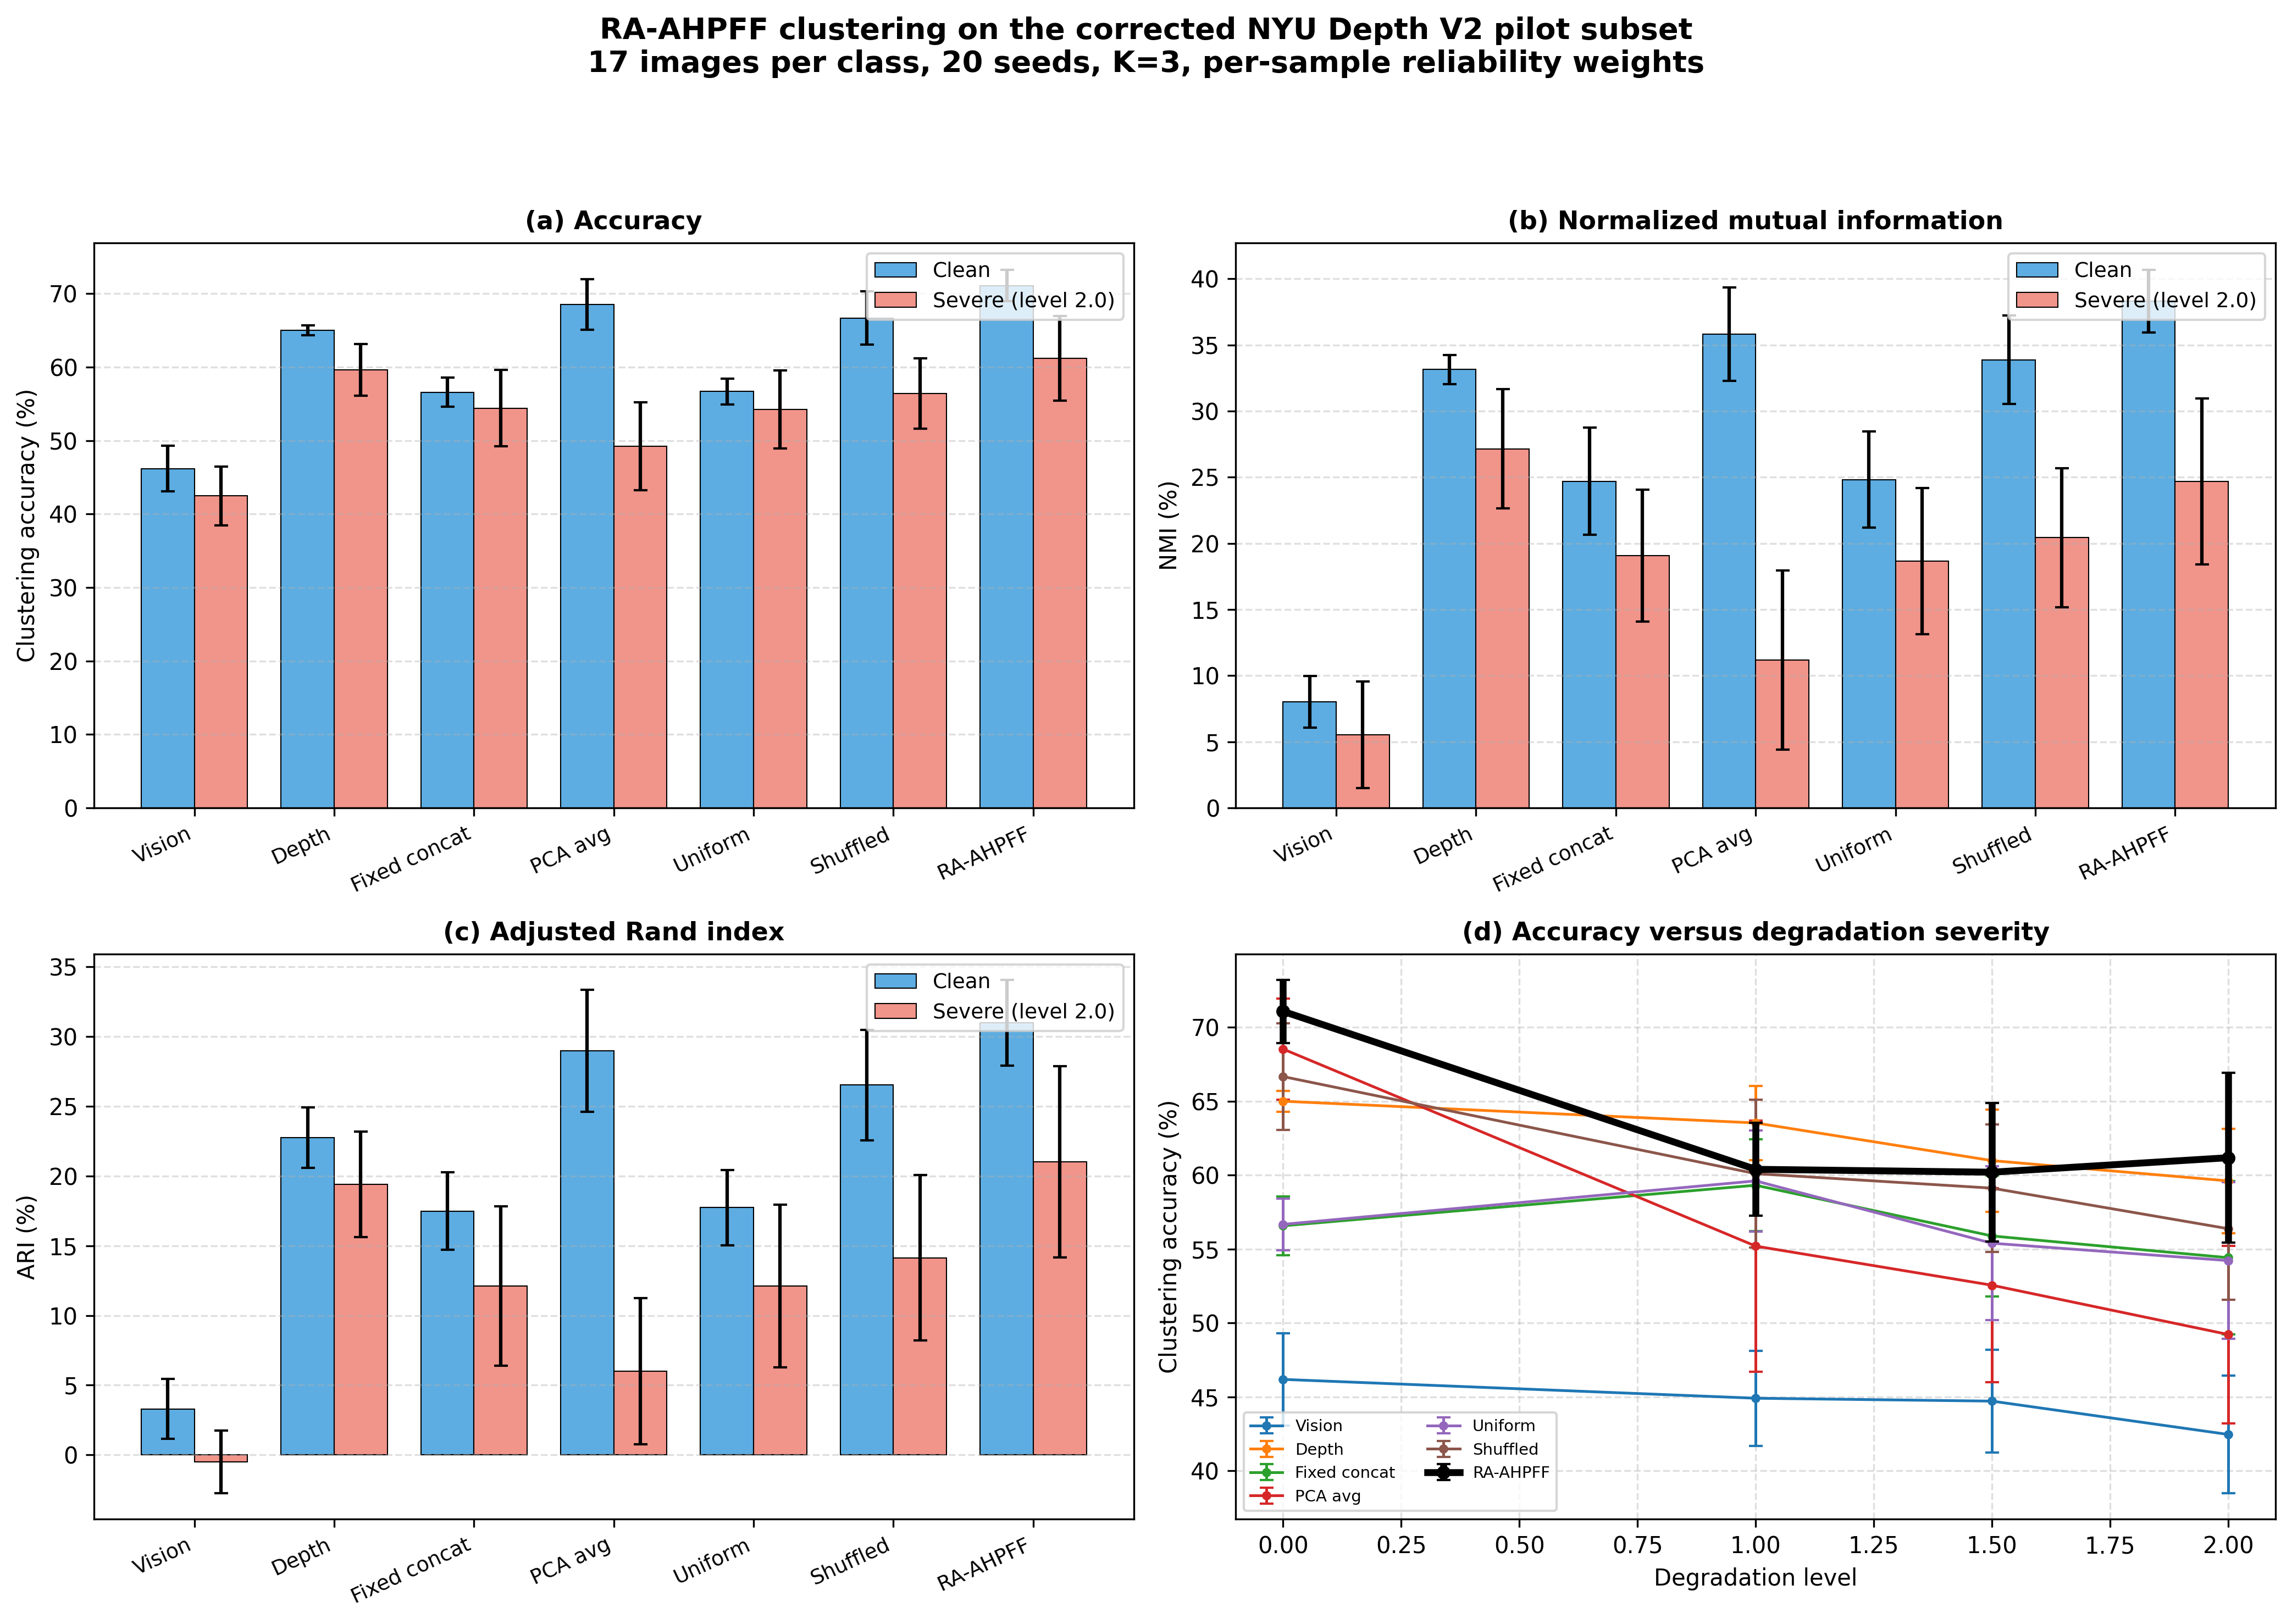
\includegraphics[width=0.92\textwidth]{ahpff_ablation.png}
    \caption{Clustering on the corrected NYU Depth V2 pilot subset. (a) ACC, (b) NMI, and (c) ARI for clean data and severe degradation (level 2.0); (d) ACC versus degradation level. All values are generated by the final benchmark code, not copied from an earlier experiment.}
    \label{fig:nyu_ablation}
\end{figure}

\subsection{In-Scene Cluster Readout and Online Accuracy}
\label{subsec:go1_cluster}
We evaluate the calibrated readout on 351 RGB-D samples collected in the Go1 street scene: Flat 59, Stairs 152, Obstacle 85, and Tactile 55. The samples are calibrated on the same scene, so this experiment measures the in-scene closed loop, not cross-domain generalization. We use two cross-validation protocols. Random 5-fold cross-validation mixes adjacent frames and therefore leaks appearance information across folds. Blocked 5-fold cross-validation sorts each class by timestamp and assigns contiguous time blocks to folds; this is the more conservative estimate. Within each blocked fold, the per-view scalers, the RW-MVK centroids, and the cluster-to-terrain mapping are fitted on the training blocks only. The held-out block is then standardized with the training scalers, assigned to the nearest centroid, and evaluated. No held-out label is used for scaling, clustering, or mapping.

\begin{table}[t]
    \centering
    \caption{In-scene terrain readout on the 351-sample Go1 calibration set. The cluster readout uses $K=32$ clusters ($r=8$) and a majority-vote cluster-to-terrain mapping. The supervised ExtraTrees model is an upper-bound comparison. Per-class recall is from the blocked protocol.}
    \label{tab:go1_cluster}
    \begin{tabular}{lcccccc}
        \toprule
        \textbf{Readout} & \textbf{Random CV} & \textbf{Blocked CV} & \textbf{Flat} & \textbf{Stairs} & \textbf{Obstacle} & \textbf{Tactile} \\
        \midrule
        Cluster readout (RA-AHPFF) & 91.2 & 77.8 & 0.44 & 0.87 & 0.79 & 0.87 \\
        Supervised ExtraTrees & 97.7 & 80.9 & 0.69 & 0.88 & 0.76 & 0.82 \\
        \bottomrule
    \end{tabular}
\end{table}

\begin{table}[t]
    \centering
    \caption{Class-wise blocked cross-validation on the 351-sample Go1 calibration set. P, R, and F1 are precision, recall, and F1-score. Balanced accuracy is the mean recall over the four classes.}
    \label{tab:go1_classwise}
    \begin{tabular}{lcccccc}
        \toprule
        & \multicolumn{3}{c}{\textbf{Cluster readout}} & \multicolumn{3}{c}{\textbf{ExtraTrees}} \\
        \cmidrule(lr){2-4}\cmidrule(lr){5-7}
        \textbf{Class} & P & R & F1 & P & R & F1 \\
        \midrule
        Flat & 0.41 & 0.44 & 0.43 & 0.52 & 0.69 & 0.59 \\
        Stairs & 0.90 & 0.87 & 0.89 & 0.88 & 0.88 & 0.88 \\
        Obstacle & 0.89 & 0.79 & 0.84 & 0.92 & 0.76 & 0.83 \\
        Tactile & 0.72 & 0.87 & 0.79 & 0.92 & 0.82 & 0.87 \\
        \midrule
        Macro avg & 0.73 & 0.74 & 0.73 & 0.81 & 0.79 & 0.79 \\
        Balanced acc & \multicolumn{3}{c}{0.74} & \multicolumn{3}{c}{0.79} \\
        \bottomrule
    \end{tabular}
\end{table}

Table~\ref{tab:go1_cluster} and Table~\ref{tab:go1_classwise} show that random cross-validation is optimistic for both readouts (91.2\% and 97.7\%), whereas the blocked protocol gives 77.8\% for the cluster readout and 80.9\% for the supervised model. The cluster readout retains most of the supervised blocked accuracy without training a discriminative classifier. The remaining gap is concentrated in the Flat class: its recall is 0.44, and the blocked confusion matrix (rows: Flat, Stairs, Obstacle, Tactile) is $[[26,9,5,19],[17,132,3,0],[13,5,67,0],[7,0,0,48]]$. Flat is therefore confused most often with Tactile (19 of 59), then Stairs (9), and only then Obstacle (5); conversely, Obstacle is most often confused with Flat (13 of 85). The low Flat recall matters for a guide dog and is discussed in Section~\ref{subsec:discussion}. This is also why we report blocked cross-validation, macro-F1, and balanced accuracy rather than only the random-CV result.

\paragraph{Zero-shot cross-illumination check.}
We also ran the model calibrated on the original street scene in a modified world with dimmer warm lighting, a darker sky, and heavier fog; the geometry and trajectory were unchanged and the model was not retrained. The online accuracy falls from 90.1\% to 73.3\%, and the Flat class is never predicted. The visual health score drops to a mean of 0.324 and the visual weight to 0.203, so the depth view dominates; the SAPF overall RMSE rises from 0.088~m to 0.149~m. This is a negative cross-domain result and confirms that the in-scene accuracy is not evidence of cross-scene generalization. A model calibrated in the target environment, or a domain-adaptation step, would be required for a new illumination condition.

In the online closed loop, the cluster readout reaches $90.1\pm1.0\%$ time-aligned semantic accuracy over three 30~s runs. This number is higher than the blocked cross-validation estimate because the deployed model is fitted on all 351 samples from the same scene, including frames from the same temporal neighbourhood; it should not be read as a cross-scene result. Under overexposure, horizontal motion blur, and 50\% depth dropout from 6 to 20~s, the online accuracy falls to $77.6\pm1.6\%$.

\subsection{Reliability Weights under Modality-Specific Degradation}
\label{subsec:weights_exp}
To verify that the weights respond to the degraded modality rather than to the terrain class alone, we ran four sessions with the same calibration model and the same trajectory: baseline, overexposure, motion blur, and depth dropout. The degradation is active from 6 to 20~s. Table~\ref{tab:weights} reports the mean weights and qualities during that window.

\begin{table}[t]
    \centering
    \caption{Mean modality weights and health qualities during the 6--20~s degradation window in the Go1 street scene. The weights are computed per sample from \eqref{eq:weights}, not set globally.}
    \label{tab:weights}
    \begin{tabular}{lcccc}
        \toprule
        \textbf{Condition} & $w_v$ & $w_d$ & $q_v$ & $q_d$ \\
        \midrule
        Baseline & 0.425 & 0.575 & 0.760 & 0.839 \\
        Overexposure & 0.174 & 0.826 & 0.442 & 0.844 \\
        Motion blur & 0.338 & 0.662 & 0.668 & 0.843 \\
        Depth dropout & 0.724 & 0.276 & 0.761 & 0.513 \\
        \bottomrule
    \end{tabular}
\end{table}

Table~\ref{tab:weights} shows the expected pattern. The visual weight drops from 0.425 at baseline to 0.174 under overexposure and to 0.338 under motion blur, while the depth weight rises correspondingly. Under depth dropout the pattern reverses: the depth weight falls to 0.276 and the visual weight rises to 0.724. The health qualities explain the weights: overexposure reduces $q_v$ from 0.760 to 0.442, and depth dropout reduces $q_d$ from 0.839 to 0.513. This is direct evidence that the per-sample reliability design responds to the degraded modality; a fixed weight or a silhouette-derived weight cannot produce this behavior.

\subsection{Reliability-to-Performance Sweep}
\label{subsec:reliability_sweep}
The weight table shows that the weights respond to degradation, but it does not by itself show that this response improves clustering. We therefore sweep one modality from clean data to severe degradation while keeping the other modality clean, and record the health score, the softmax weight, and the clustering accuracy/NMI. The sweep uses the 51-image NYU pilot set, $K=3$, $\lambda=4$, and 20 seeds; each level degrades all samples of the selected modality.

\begin{figure}[t]
    \centering
    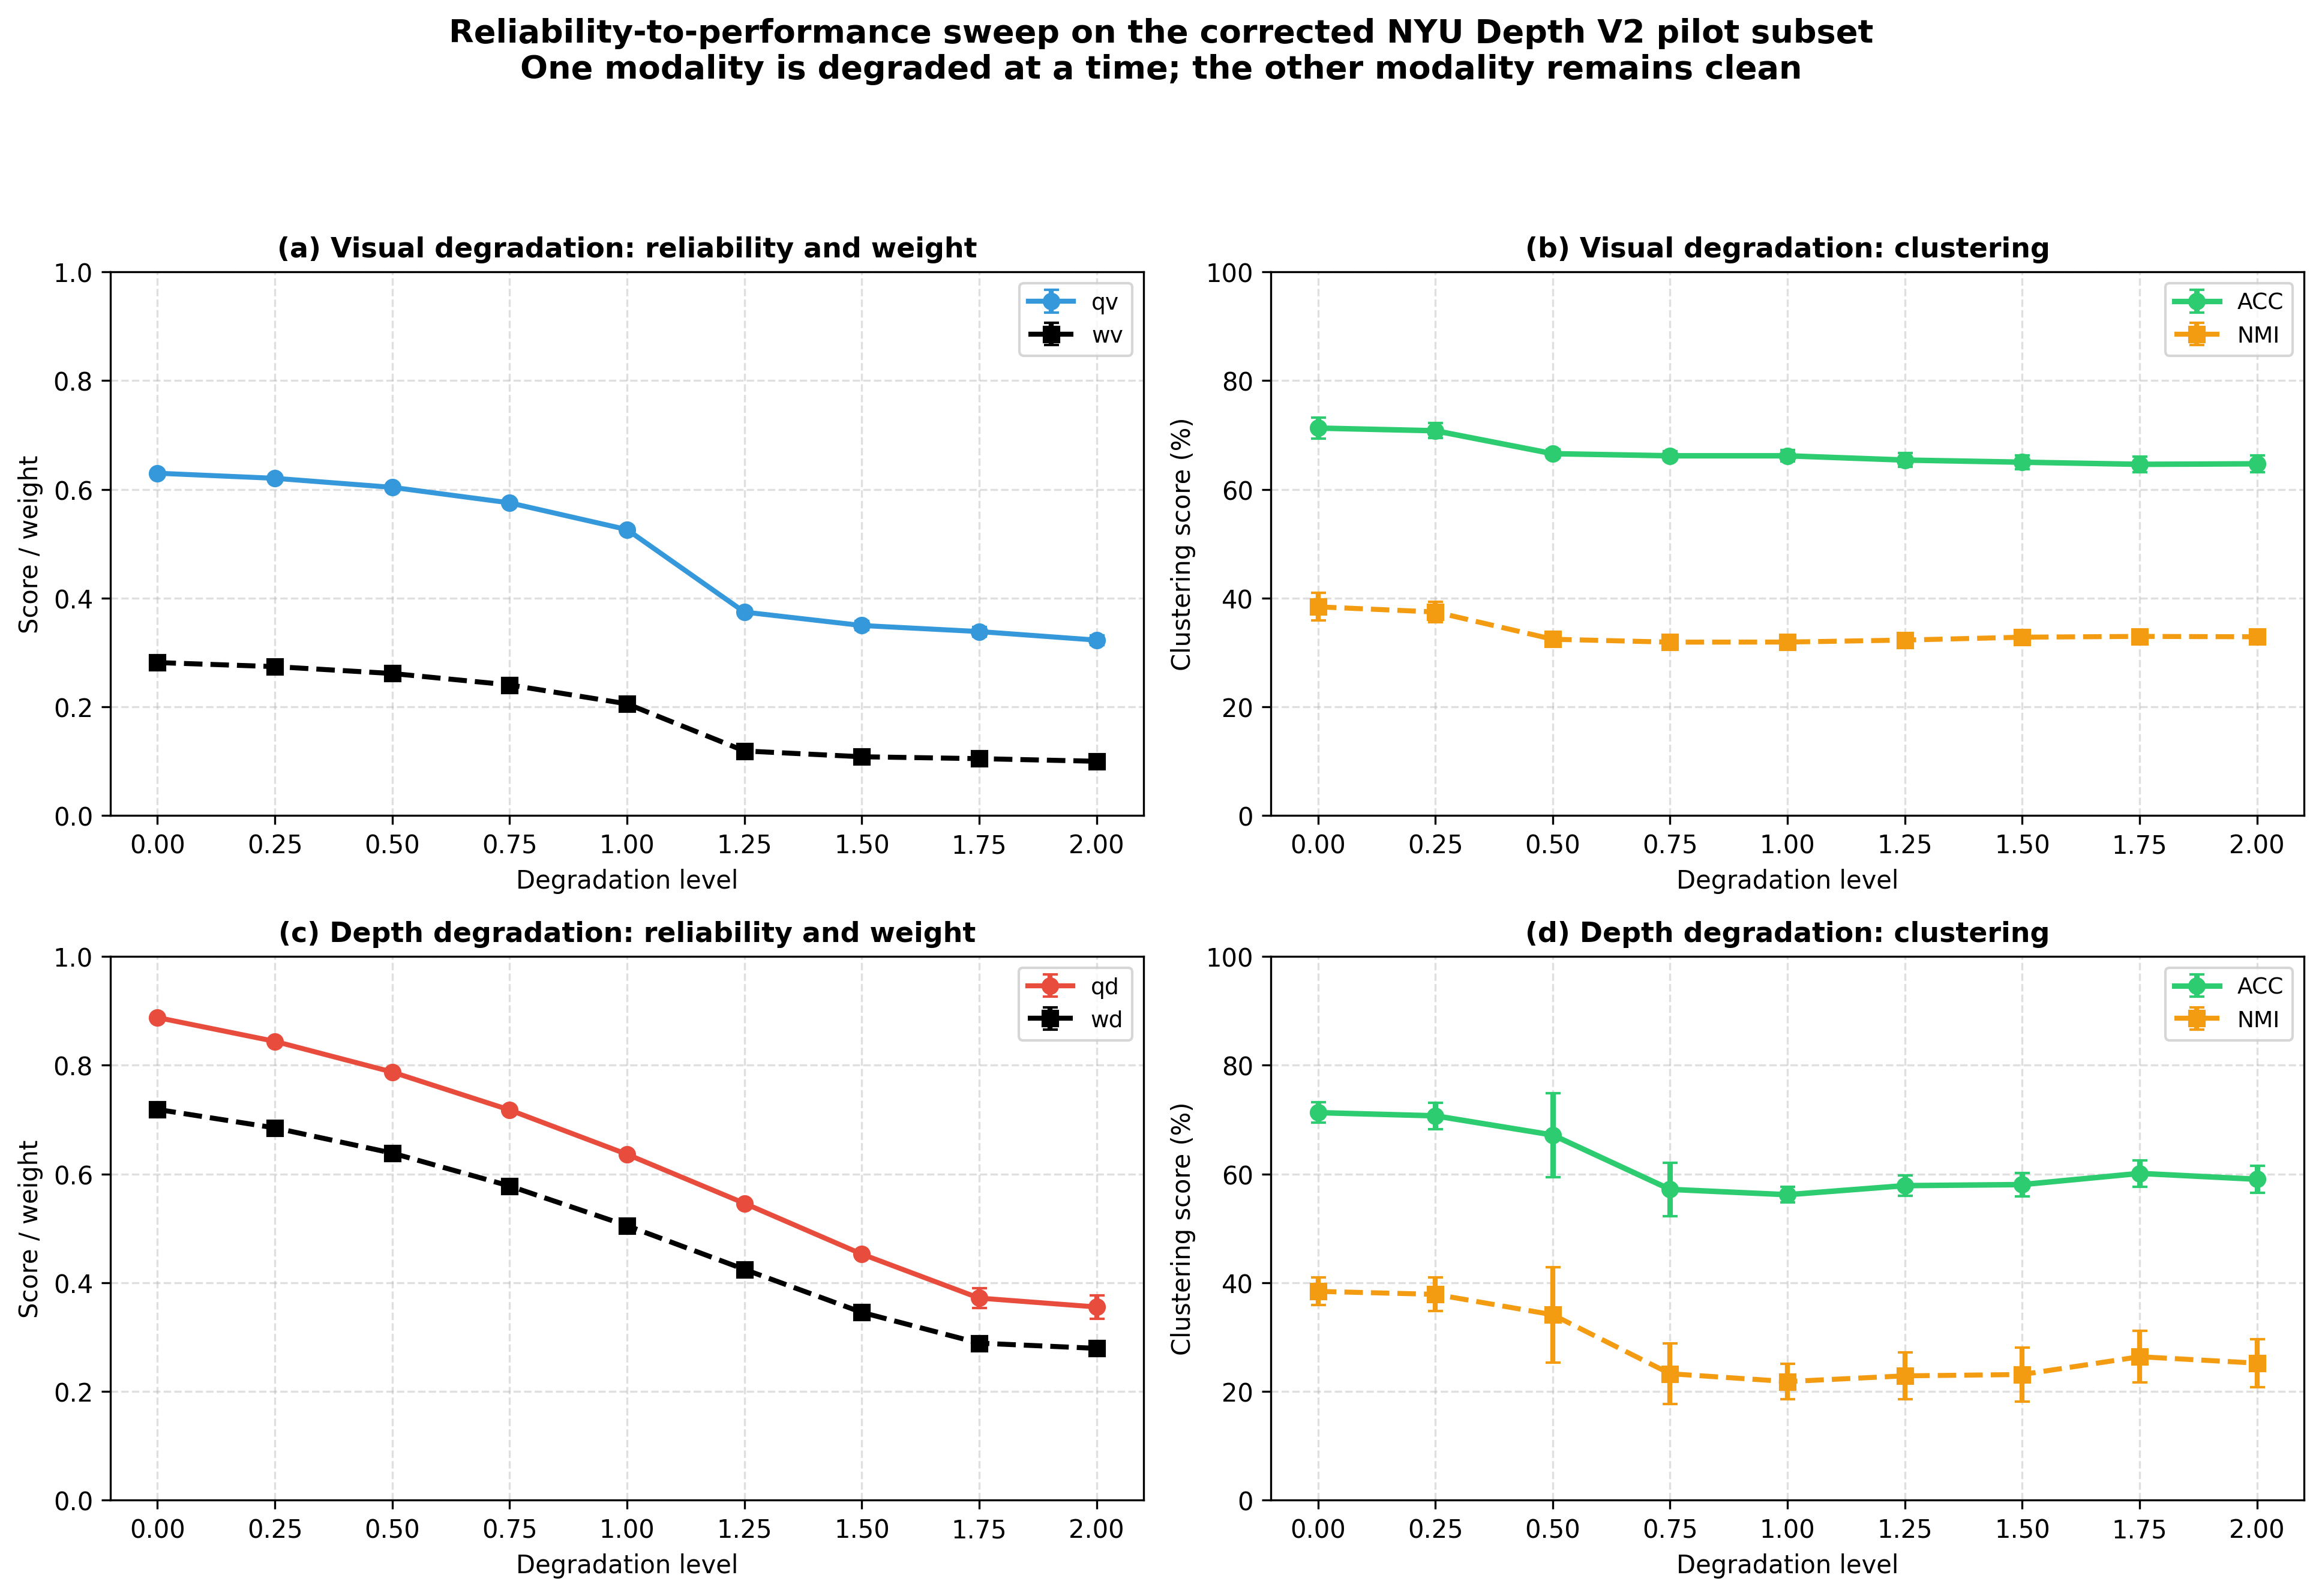
\includegraphics[width=0.92\textwidth]{reliability_sweep.png}
    \caption{Reliability-to-performance sweep on the NYU pilot subset. (a) Visual degradation lowers $q_v$ and $w_v$. (b) Clustering accuracy and NMI decrease as the visual stream degrades. (c) Depth degradation lowers $q_d$ and $w_d$. (d) Clustering accuracy and NMI decrease as the depth stream degrades. The depth sweep is non-monotonic at high levels because the depth contribution is strongly downweighted and the clean visual view dominates.}
    \label{fig:reliability_sweep}
\end{figure}

For the visual sweep, $q_v$ falls from 0.630 to 0.323 and $w_v$ falls from 0.281 to 0.100; accuracy falls from 71.3\% to 64.7\% and NMI from 38.4\% to 32.9\%. For the depth sweep, $q_d$ falls from 0.888 to 0.355 and $w_d$ falls from 0.719 to 0.279; accuracy falls from 71.3\% to 59.0\% and NMI from 38.4\% to 25.2\%. The depth sweep is not strictly monotonic: after an initial drop, the accuracy partially recovers as the depth weight becomes small and the clean visual view takes over. This is consistent with the weighting mechanism, but it also shows that the reliability score is a quality indicator, not a direct performance predictor. The important point is that the degradation, reliability score, modality weight, and clustering performance move together in the expected direction.

\subsection{Semantic-Adaptive Particle Filter: Fair Comparison}
\label{subsec:sapf_exp}
We first evaluate the filters on a standalone 30~s stair-climbing simulation with 20 seeds. The trajectory contains flat ground, an obstacle, and a staircase; odometry has a small vertical bias on stairs. The semantic labels come from the three-class cluster readout fitted on the corrected NYU pilot set (holdout accuracy 66.7\%, sequence semantic accuracy 73.0\%). The exteroceptive pose is available at 5~Hz with the same two outage windows as the Gazebo study. The compared methods are leg odometry (LO), the standard particle filter (SPF), the fixed large-covariance particle filter (LPF), an extended Kalman filter (EKF), SAPF with predicted labels, SAPF with oracle labels, and SAPF with shuffled predicted labels. All particle filters use 1000 particles and the same odometry and observation streams.

\begin{table}[t]
    \centering
    \caption{Standalone 6-DoF stair-climbing simulation over 20 seeds (1000 particles). Values are mean RMSE in metres (orientation in radians). The sequence semantic accuracy of the cluster readout is 73.0\%.}
    \label{tab:standalone_sapf}
    \begin{tabular}{lcccc}
        \toprule
        \textbf{Method} & \textbf{$Z$ RMSE} & \textbf{Position RMSE} & \textbf{Orientation RMSE} & \textbf{Stairs $Z$ RMSE} \\
        \midrule
        LO & 0.2960 & 0.3456 & 0.0935 & 0.3342 \\
        SPF & 0.2597 & 0.2647 & 0.0291 & 0.3141 \\
        LPF & \textbf{0.0992} & \textbf{0.1107} & 0.0283 & 0.1478 \\
        EKF & 0.1670 & 0.1734 & 0.0257 & 0.2476 \\
        SAPF-Pred & 0.1062 & 0.1158 & 0.0264 & 0.1552 \\
        SAPF-Oracle & 0.1014 & 0.1123 & 0.0268 & 0.1426 \\
        SAPF-Shuffled & 0.1295 & 0.1374 & 0.0261 & 0.1920 \\
        \bottomrule
    \end{tabular}
\end{table}

\begin{figure}[t]
    \centering
    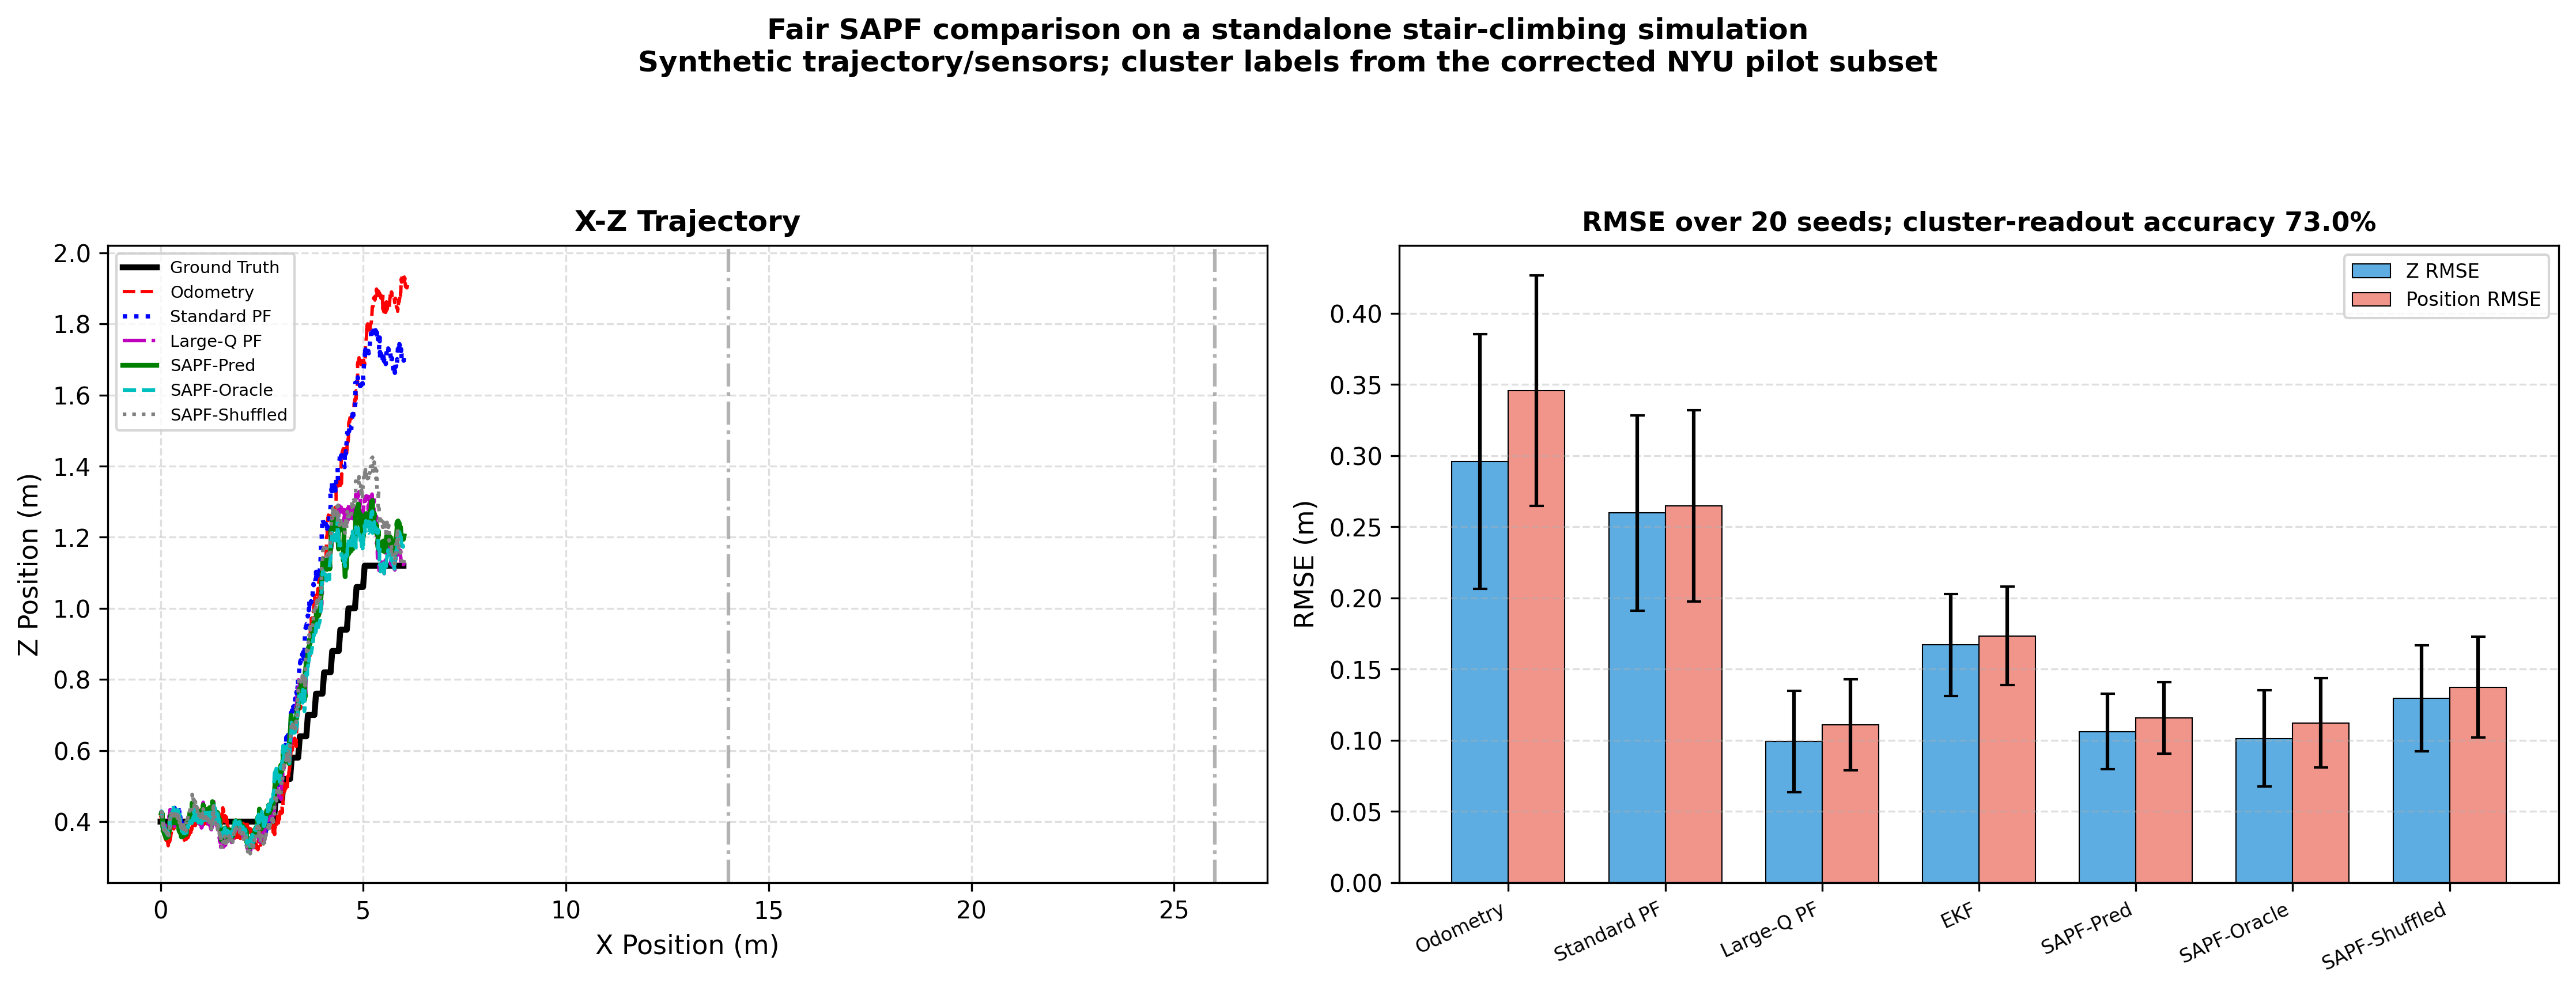
\includegraphics[width=0.92\textwidth]{sapf_tracking_result.png}
    \caption{Standalone SAPF comparison over 20 seeds. The large-covariance PF is a strong baseline; the predicted-label SAPF is close to it, and the shuffled-label control is worse.}
    \label{fig:sapf_standalone}
\end{figure}

Fig.~\ref{fig:sapf_standalone} and Table~\ref{tab:standalone_sapf} show the standalone results, which are deliberately sobering. The large fixed covariance LPF is a very strong baseline (0.1107~m position RMSE), and the predicted-label SAPF is close to it (0.1158~m). The oracle-label SAPF is slightly better (0.1123~m), and the shuffled-label SAPF is clearly worse (0.1374~m). The semantic label therefore carries information, but a globally inflated covariance can recover much of the benefit when the exteroceptive pose is reasonably accurate. We do not claim that semantic adaptation alone explains the improvement over the standard PF.

Fig.~\ref{fig:trajectory} and Fig.~\ref{fig:semantic_labels} show a representative trajectory and label stream. We then repeat the closed-loop Go1 experiment three times with different random seeds, using the same 5~Hz observation schedule and outages. Table~\ref{tab:go1_sapf} reports the mean and standard deviation. The semantic accuracy is $90.1\pm1.0\%$ at baseline and $77.6\pm1.6\%$ under the mixed degradation. The SPF remains poor in both conditions (0.1711~m and 0.1726~m overall), while the LPF and SAPF are both around 0.09~m. The SAPF is comparable to the LPF at baseline (0.0877~m versus 0.0883~m) and slightly worse under degradation (0.0958~m versus 0.0937~m). The shuffled-label control is worse at baseline (0.1131~m) and close to the SAPF under degradation (0.0999~m), which indicates that the terrain label is useful mainly when the label stream is reliable.

\begin{table}[t]
    \centering
    \caption{Go1 closed-loop pose RMSE over three 30~s runs. Values are mean$\pm$standard deviation in metres. The exteroceptive pose is available at 5~Hz with two 4~s outages.}
    \label{tab:go1_sapf}
    \resizebox{\textwidth}{!}{%
    \begin{tabular}{lcccc}
        \toprule
        & \multicolumn{2}{c}{\textbf{Baseline}} & \multicolumn{2}{c}{\textbf{Degraded}} \\
        \cmidrule(lr){2-3}\cmidrule(lr){4-5}
        \textbf{Method} & Overall & $Z$ & Overall & $Z$ \\
        \midrule
        LO & 0.2520$\pm$0.0607 & 0.1861$\pm$0.0684 & 0.2592$\pm$0.0649 & 0.1819$\pm$0.0824 \\
        SPF & 0.1711$\pm$0.0313 & 0.1593$\pm$0.0350 & 0.1726$\pm$0.0289 & 0.1607$\pm$0.0337 \\
        LPF & 0.0883$\pm$0.0078 & \textbf{0.0640$\pm$0.0049} & \textbf{0.0937$\pm$0.0107} & \textbf{0.0721$\pm$0.0120} \\
        EKF & 0.1285$\pm$0.0113 & 0.1153$\pm$0.0122 & 0.1267$\pm$0.0110 & 0.1131$\pm$0.0152 \\
        SAPF-Pred & \textbf{0.0877$\pm$0.0080} & 0.0663$\pm$0.0088 & 0.0958$\pm$0.0127 & 0.0762$\pm$0.0151 \\
        SAPF-Oracle & 0.1015$\pm$0.0098 & 0.0829$\pm$0.0071 & 0.1137$\pm$0.0157 & 0.0962$\pm$0.0197 \\
        SAPF-Shuffled & 0.1131$\pm$0.0031 & 0.0979$\pm$0.0080 & 0.0999$\pm$0.0134 & 0.0830$\pm$0.0158 \\
        \bottomrule
    \end{tabular}}
\end{table}

The oracle-label SAPF is not uniformly the best in Table~\ref{tab:go1_sapf}. This is not a contradiction: the filter performance depends on when the uncertainty is inflated, not only on whether the class is correct at the current instant. A label stream that anticipates a transition can be more useful than an exact but late label, and the predicted stream is smoothed over five frames. We therefore use the shuffled-label control, not the oracle, as the main evidence that terrain timing matters; the control preserves the label distribution but destroys the temporal correspondence.

\begin{figure}[t]
    \centering
    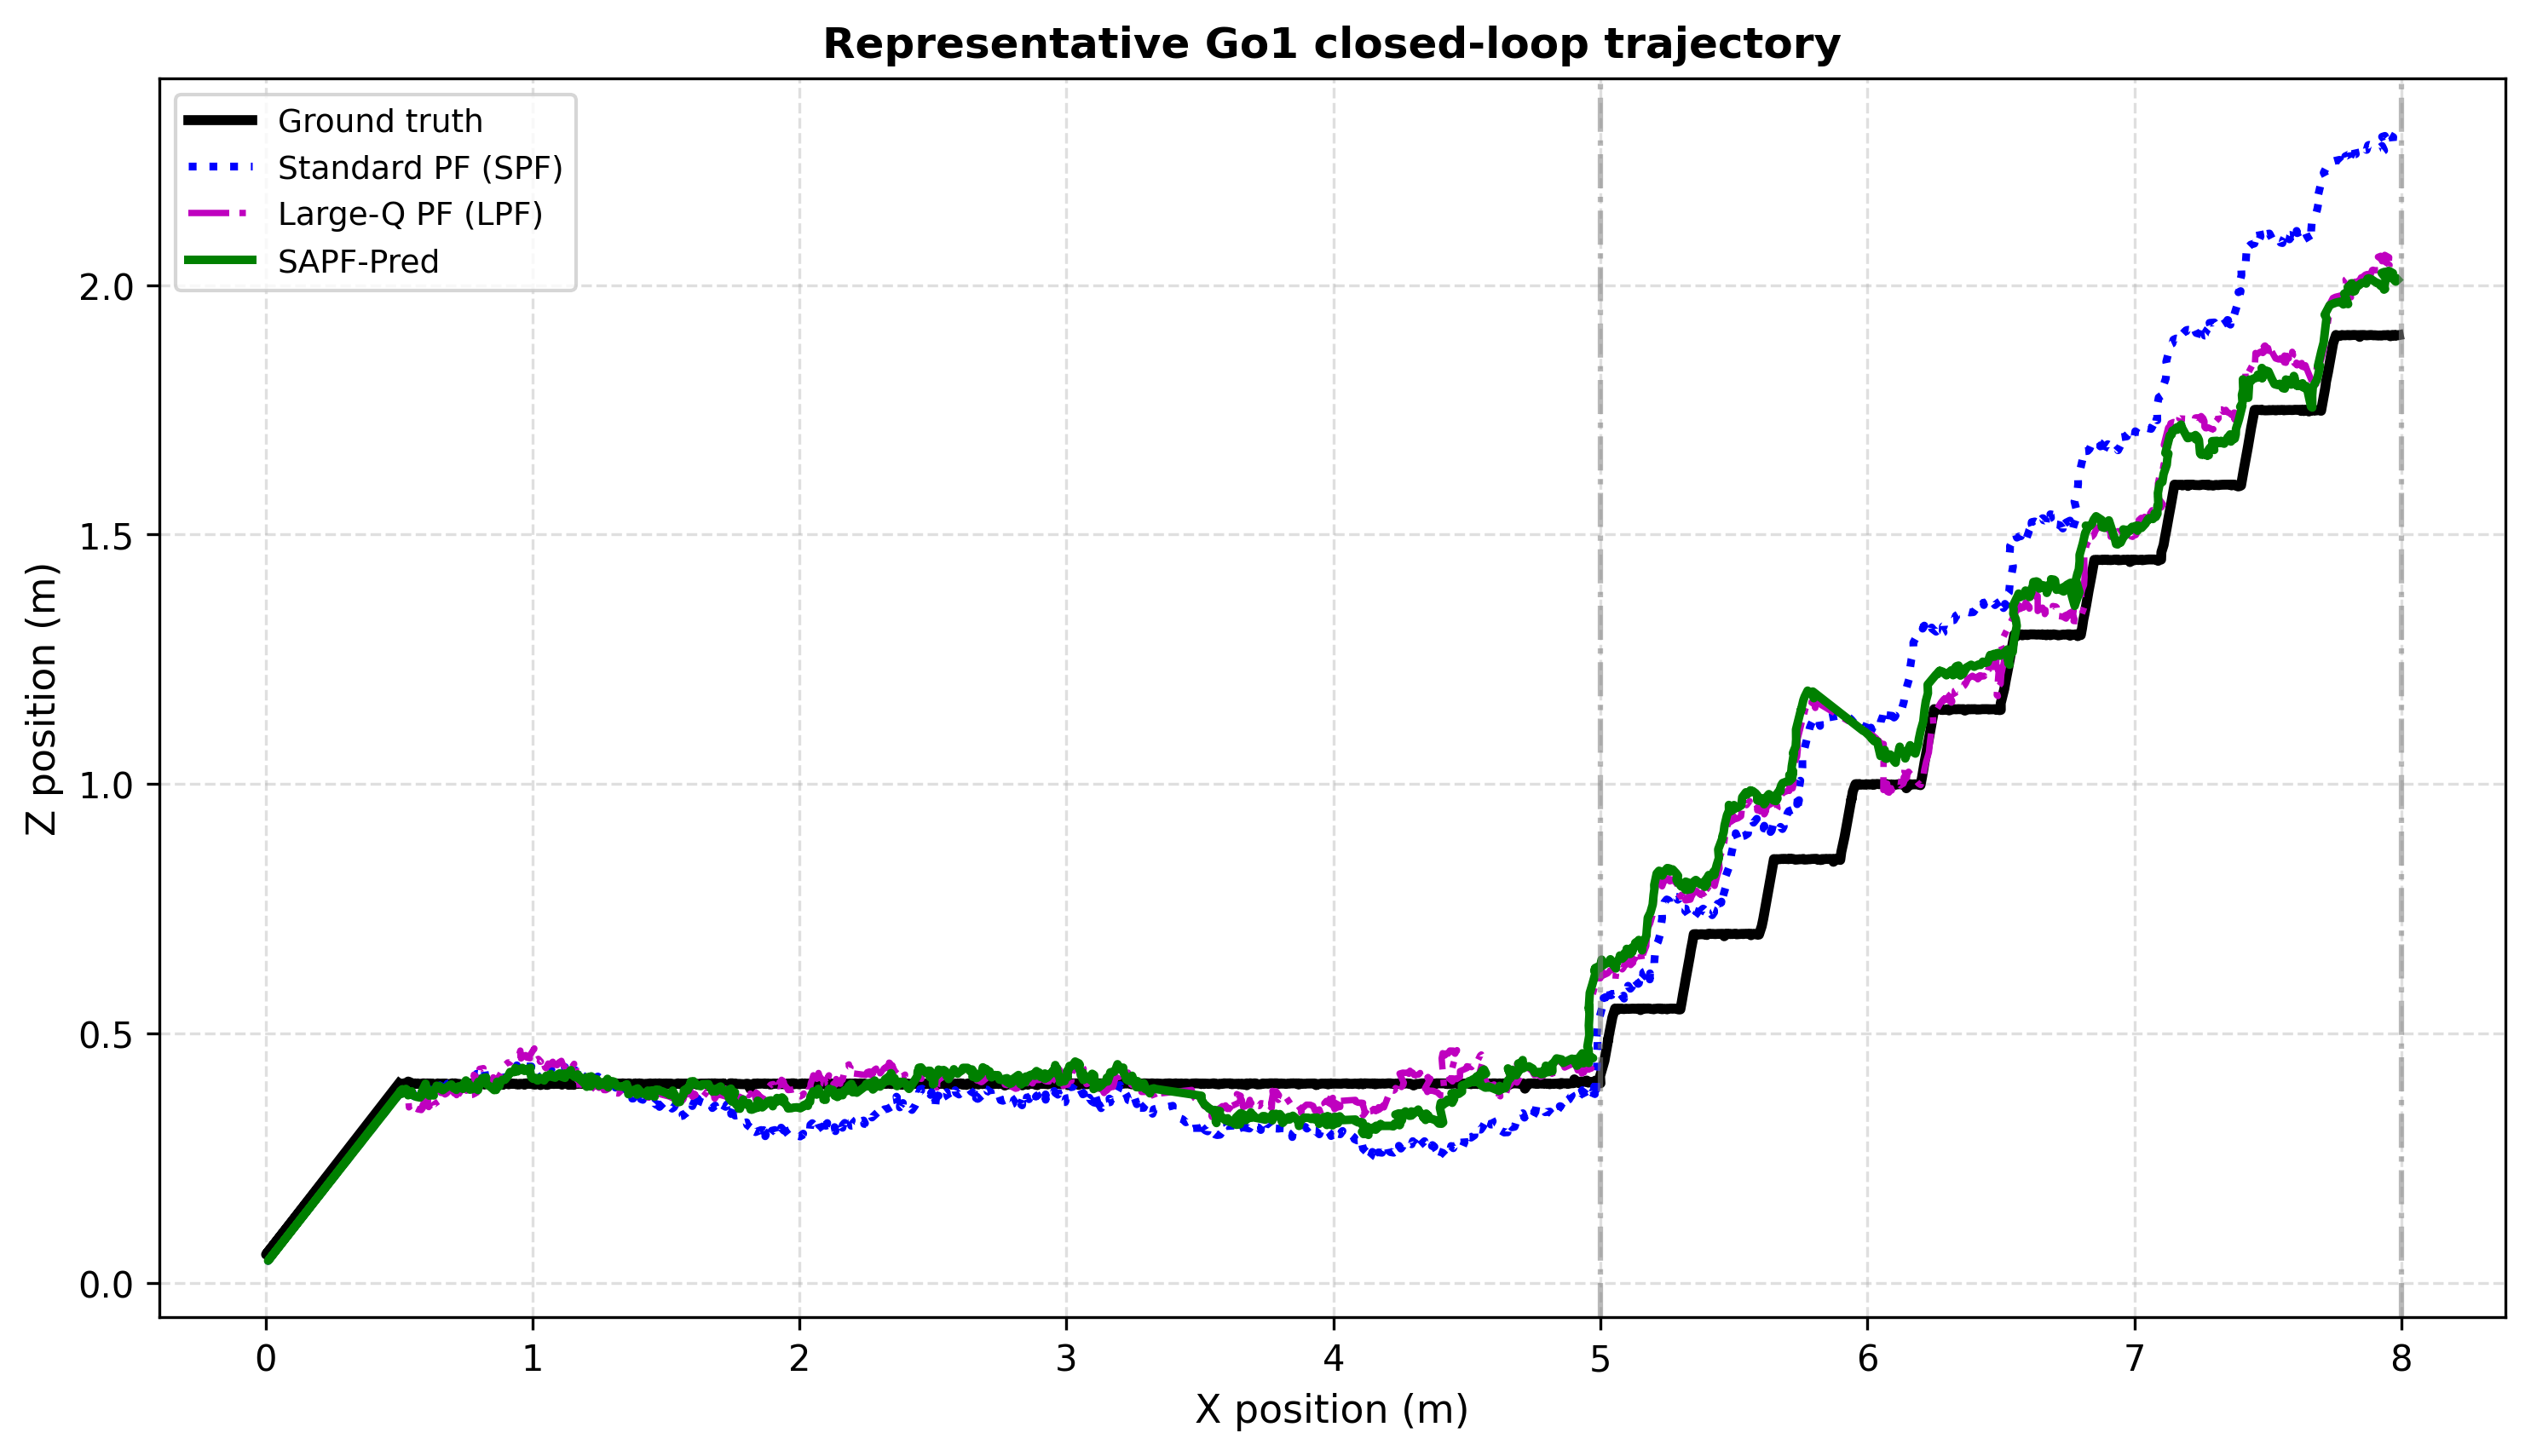
\includegraphics[width=0.82\textwidth]{trajectory_lpf_sapf.png}
    \caption{X--Z trajectory in the Go1 closed-loop study (representative baseline run). Only the trajectories used in the fair comparison are shown; the oracle and shuffled variants are reported numerically in Table~\ref{tab:go1_sapf}. The standard PF lags on the staircase, while the large-covariance PF and SAPF-Pred track the elevation.}
    \label{fig:trajectory}
\end{figure}

\begin{figure}[t]
    \centering
    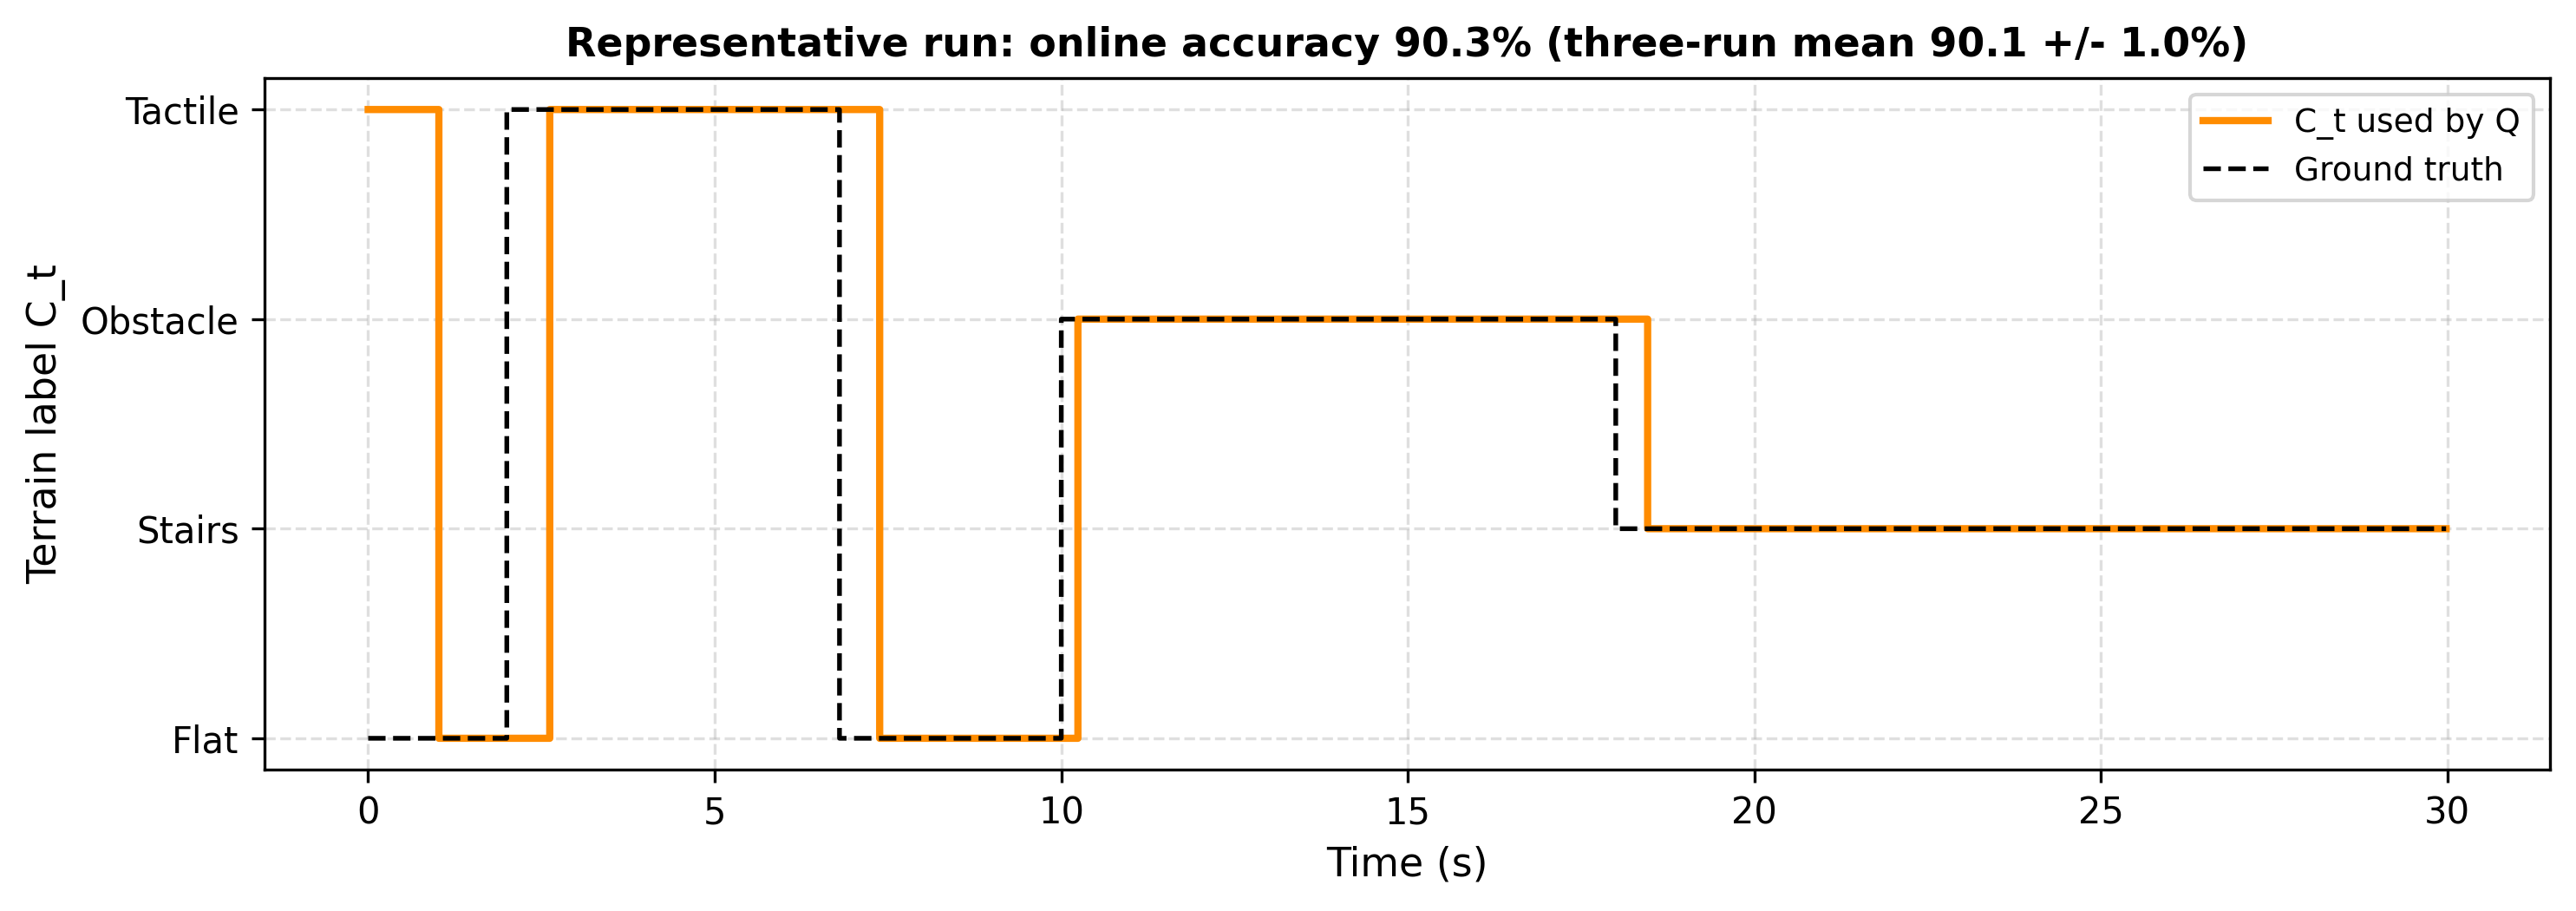
\includegraphics[width=0.82\textwidth]{semantic_labels_representative.png}
    \caption{Terrain label $C_t$ used by the SAPF versus the scripted ground-truth label in a representative baseline run (online accuracy 90.3\%). The mean over three runs is 90.1$\pm$1.0\% time-aligned accuracy.}
    \label{fig:semantic_labels}
\end{figure}

\subsection{Discussion and Limitations}
\label{subsec:discussion}
The experiments support a narrow claim: reliability-aware clustering is a practical way to obtain online terrain labels for a guide-dog robot when the camera or depth stream degrades, and the resulting labels are useful to a downstream filter. The evidence also shows the limits of the claim. First, the NYU study is a 51-image pilot subset; the confidence intervals are wide and depth-only clustering is competitive at mild degradation. Second, the in-scene readout is calibrated on the same Gazebo scene, and the blocked cross-validation estimate (77.8\%) is lower than the online accuracy (90.1\%) precisely because the online model sees the whole scene; a zero-shot cross-illumination run on the same geometry falls to 73.3\%. Third, the large-covariance PF is a strong baseline; semantic adaptation is comparable rather than dramatically better, and the oracle-label variant is not uniformly best. Fourth, the Gazebo observation is a simulated exteroceptive pose at 5~Hz with outages, and the Go1 motion is kinematic; the study does not demonstrate a physics-based gait or a real-world deployment. Fifth, the health coefficients and the over-clustering factors are fixed calibration parameters, not learned end-to-end. Sixth, the online readout still has a low Flat recall (0.44), a macro-F1 of 0.73, and a balanced accuracy of 0.74; Table~\ref{tab:go1_classwise} shows that Flat is confused mainly with Tactile and Stairs. This matters because false obstacle or stair labels can cause unnecessary stops or detours for a guide dog.


%% ==========================================
%% 5. Conclusion
%% ==========================================
\section{Conclusion}
\label{sec:conclusion}
We presented a reliability-aware RGB-D terrain clustering front end for robotic guide dogs and connected it to a 6-DoF semantic-adaptive particle filter. The method replaces silhouette-derived fusion weights with per-sample sensor-health weights, uses weighted concatenation instead of adding PCA coordinates from different sensor spaces, and calibrates cluster indices to terrain classes so that clustering is used online. On a corrected NYU pilot subset, the method has the best clean accuracy and the numerically highest accuracy at severe degradation, and the weights respond correctly to visually and depth-degraded samples. In a Go1 Gazebo street scene, the cluster readout reaches 90.1\% online accuracy and 77.8\% under blocked cross-validation, compared with 80.9\% for a supervised upper bound; under mixed sensor degradation the online accuracy falls to 77.6\%, while the SAPF remains close to a strong large-covariance baseline and clearly improves over the standard particle filter. The study is limited by the small NYU subset, kinematic Gazebo locomotion, a simulated exteroceptive pose, in-scene calibration, and a zero-shot cross-illumination drop to 73.3\%. Future work will (i) evaluate the method on a larger multi-scene RGB-D terrain dataset, including outdoor LiDAR data such as SemanticKITTI \cite{behley2019semantickitti}, (ii) integrate a physics-based locomotion controller, and (iii) test the cluster readout on a physical quadrupedal platform.

\section*{Acknowledgments}
This work was supported by the Special Environment Robotics Laboratory at Southwest University of Science and Technology.

%% ==========================================
%% References
%% ==========================================
\bibliographystyle{elsarticle-num}
\bibliography{refs}

\end{document}
